% GNUPLOT: LaTeX picture with Postscript
\begingroup
  \makeatletter
  \providecommand\color[2][]{%
    \GenericError{(gnuplot) \space\space\space\@spaces}{%
      Package color not loaded in conjunction with
      terminal option `colourtext'%
    }{See the gnuplot documentation for explanation.%
    }{Either use 'blacktext' in gnuplot or load the package
      color.sty in LaTeX.}%
    \renewcommand\color[2][]{}%
  }%
  \providecommand\includegraphics[2][]{%
    \GenericError{(gnuplot) \space\space\space\@spaces}{%
      Package graphicx or graphics not loaded%
    }{See the gnuplot documentation for explanation.%
    }{The gnuplot epslatex terminal needs graphicx.sty or graphics.sty.}%
    \renewcommand\includegraphics[2][]{}%
  }%
  \providecommand\rotatebox[2]{#2}%
  \@ifundefined{ifGPcolor}{%
    \newif\ifGPcolor
    \GPcolorfalse
  }{}%
  \@ifundefined{ifGPblacktext}{%
    \newif\ifGPblacktext
    \GPblacktexttrue
  }{}%
  % define a \g@addto@macro without @ in the name:
  \let\gplgaddtomacro\g@addto@macro
  % define empty templates for all commands taking text:
  \gdef\gplbacktext{}%
  \gdef\gplfronttext{}%
  \makeatother
  \ifGPblacktext
    % no textcolor at all
    \def\colorrgb#1{}%
    \def\colorgray#1{}%
  \else
    % gray or color?
    \ifGPcolor
      \def\colorrgb#1{\color[rgb]{#1}}%
      \def\colorgray#1{\color[gray]{#1}}%
      \expandafter\def\csname LTw\endcsname{\color{white}}%
      \expandafter\def\csname LTb\endcsname{\color{black}}%
      \expandafter\def\csname LTa\endcsname{\color{black}}%
      \expandafter\def\csname LT0\endcsname{\color[rgb]{1,0,0}}%
      \expandafter\def\csname LT1\endcsname{\color[rgb]{0,1,0}}%
      \expandafter\def\csname LT2\endcsname{\color[rgb]{0,0,1}}%
      \expandafter\def\csname LT3\endcsname{\color[rgb]{1,0,1}}%
      \expandafter\def\csname LT4\endcsname{\color[rgb]{0,1,1}}%
      \expandafter\def\csname LT5\endcsname{\color[rgb]{1,1,0}}%
      \expandafter\def\csname LT6\endcsname{\color[rgb]{0,0,0}}%
      \expandafter\def\csname LT7\endcsname{\color[rgb]{1,0.3,0}}%
      \expandafter\def\csname LT8\endcsname{\color[rgb]{0.5,0.5,0.5}}%
    \else
      % gray
      \def\colorrgb#1{\color{black}}%
      \def\colorgray#1{\color[gray]{#1}}%
      \expandafter\def\csname LTw\endcsname{\color{white}}%
      \expandafter\def\csname LTb\endcsname{\color{black}}%
      \expandafter\def\csname LTa\endcsname{\color{black}}%
      \expandafter\def\csname LT0\endcsname{\color{black}}%
      \expandafter\def\csname LT1\endcsname{\color{black}}%
      \expandafter\def\csname LT2\endcsname{\color{black}}%
      \expandafter\def\csname LT3\endcsname{\color{black}}%
      \expandafter\def\csname LT4\endcsname{\color{black}}%
      \expandafter\def\csname LT5\endcsname{\color{black}}%
      \expandafter\def\csname LT6\endcsname{\color{black}}%
      \expandafter\def\csname LT7\endcsname{\color{black}}%
      \expandafter\def\csname LT8\endcsname{\color{black}}%
    \fi
  \fi
  \setlength{\unitlength}{0.0500bp}%
  \begin{picture}(7600.00,5700.00)%
      \put(500,2600){\makebox(0,0)[r]{\strut{}$\mathbf{n=3}$}}%
      \put(858,440){\makebox(0,0)[r]{\strut{} 0}}%
      \put(858,1045){\makebox(0,0)[r]{\strut{} 0.15}}%
      \put(858,1651){\makebox(0,0)[r]{\strut{} 0.3}}%
      \put(858,2256){\makebox(0,0)[r]{\strut{} 0.45}}%
      \put(990,220){\makebox(0,0){\strut{}-5}}%
      \put(1543,220){\makebox(0,0){\strut{}-2.5}}%
      \put(2097,220){\makebox(0,0){\strut{} 0}}%
      \put(2650,220){\makebox(0,0){\strut{} 2.5}}%
      \put(3203,220){\makebox(0,0){\strut{} 5}}%
      \put(1100,2083){\makebox(0,0)[l]{\strut{}sum}}%
      \put(1100,1863){\makebox(0,0)[l]{\strut{}gaussian}}%
          \put(0,0){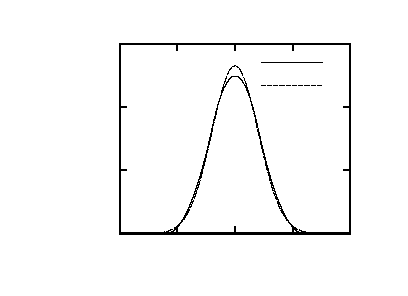
\includegraphics{conv_2}}%

      \put(4500,2600){\makebox(0,0)[r]{\strut{}$\mathbf{n=7}$}}%
      \put(4858,440){\makebox(0,0)[r]{\strut{} 0}}%
      \put(4858,1045){\makebox(0,0)[r]{\strut{} 0.15}}%
      \put(4858,1651){\makebox(0,0)[r]{\strut{} 0.3}}%
      \put(4858,2256){\makebox(0,0)[r]{\strut{} 0.45}}%
      \put(4990,220){\makebox(0,0){\strut{}-5}}%
      \put(5543,220){\makebox(0,0){\strut{}-2.5}}%
      \put(6097,220){\makebox(0,0){\strut{} 0}}%
      \put(6650,220){\makebox(0,0){\strut{} 2.5}}%
      \put(7203,220){\makebox(0,0){\strut{} 5}}%
      \put(5100,2083){\makebox(0,0)[l]{\strut{}sum}}%
      \put(5100,1863){\makebox(0,0)[l]{\strut{}gaussian}}%
          \put(4000,0){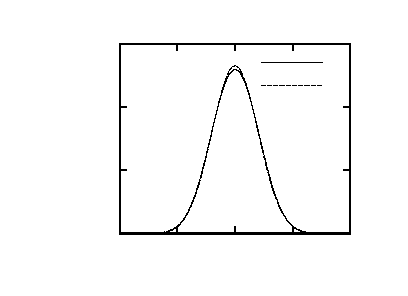
\includegraphics{conv_6}}%

      \put(500,5600){\makebox(0,0)[r]{\strut{}$\mathbf{n=1}$}}%
      \put(858,3440){\makebox(0,0)[r]{\strut{} 0}}%
      \put(858,4045){\makebox(0,0)[r]{\strut{} 0.15}}%
      \put(858,4651){\makebox(0,0)[r]{\strut{} 0.3}}%
      \put(858,5256){\makebox(0,0)[r]{\strut{} 0.45}}%
      \put(990,3220){\makebox(0,0){\strut{}-5}}%
      \put(1543,3220){\makebox(0,0){\strut{}-2.5}}%
      \put(2097,3220){\makebox(0,0){\strut{} 0}}%
      \put(2650,3220){\makebox(0,0){\strut{} 2.5}}%
      \put(3203,3220){\makebox(0,0){\strut{} 5}}%
      \put(1100,5083){\makebox(0,0)[l]{\strut{}sum}}%
      \put(1100,4863){\makebox(0,0)[l]{\strut{}gaussian}}%
          \put(0,3000){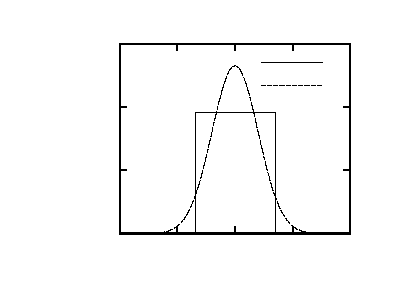
\includegraphics{conv_0}}%

      \put(4500,5600){\makebox(0,0)[r]{\strut{}$\mathbf{n=2}$}}%
      \put(4858,3440){\makebox(0,0)[r]{\strut{} 0}}%
      \put(4858,4045){\makebox(0,0)[r]{\strut{} 0.15}}%
      \put(4858,4651){\makebox(0,0)[r]{\strut{} 0.3}}%
      \put(4858,5256){\makebox(0,0)[r]{\strut{} 0.45}}%
      \put(4990,3220){\makebox(0,0){\strut{}-5}}%
      \put(5543,3220){\makebox(0,0){\strut{}-2.5}}%
      \put(6097,3220){\makebox(0,0){\strut{} 0}}%
      \put(6650,3220){\makebox(0,0){\strut{} 2.5}}%
      \put(7203,3220){\makebox(0,0){\strut{} 5}}%
      \put(5100,5083){\makebox(0,0)[l]{\strut{}sum}}%
      \put(5100,4863){\makebox(0,0)[l]{\strut{}gaussian}}%
          \put(4000,3000){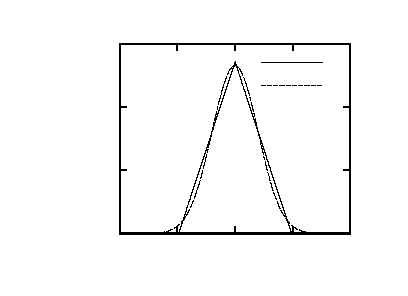
\includegraphics{conv_1}}%



  \end{picture}%
\endgroup
